
\documentclass{beamer}
\usecolortheme{dove}
\setbeamertemplate{navigation symbols}{}
\usepackage{amsmath,amssymb,amsfonts,amsthm, multicol, subfigure, color}
\usepackage{bm}
\usepackage{graphicx}
\usepackage{tabularx}
\usepackage{booktabs}
\usepackage{hyperref}
\usepackage{pdfpages}
\usepackage{xcolor}
\definecolor{seagreen}{RGB}{46, 139, 87}
\def\independenT#1#2{\mathrel{\rlap{$#1#2$}\mkern2mu{#1#2}}}
\newcommand\indep{\protect\mathpalette{\protect\independenT}{\perp}}
\def\log{\text{log}}
\newcommand\logit{\text{logit}}
\newcommand\iid{\stackrel{\text{iid}}{\sim}}
\newcommand\E{\text{E}}
\newcommand\V{\text{V}}
\renewcommand\P{\text{P}}
\newcommand{\Cov}{\text{Cov}}
\newcommand{\Cor}{\text{Cor}}
\newcommand\doop{\texttt{do}}
\usepackage{stackrel}
\usepackage{tikz}
\usetikzlibrary{arrows,shapes.arrows,positioning,shapes,patterns,calc}
\newcommand\slideref[1]{\vskip .1cm \tiny \textcolor{gray}{{#1}}}
\newcommand\red[1]{\color{red}#1}
\newcommand\blue[1]{\color{blue}#1}
\newcommand\gray[1]{\color{gray}#1}
\newcommand\seagreen[1]{\color{seagreen}#1}
\newcommand\purple[1]{\color{purple}#1}
\newcommand\orange[1]{\color{orange}#1}
\newcommand\black[1]{\color{black}#1}
\newcommand\white[1]{\color{white}#1}
\newcommand\teal[1]{\color{teal}#1}
\newcommand\magenta[1]{\color{magenta}#1}
\newcommand\Fuchsia[1]{\color{Fuchsia}#1}
\newcommand\BlueGreen[1]{\color{BlueGreen}#1}
\newcommand\bblue[1]{\textcolor{blue}{\textbf{#1}}}
\newcommand\bred[1]{\textcolor{red}{\textbf{#1}}}
\newcommand\bgray[1]{\textcolor{gray}{\textbf{#1}}}
\newcommand\bgreen[1]{\textcolor{seagreen}{\textbf{#1}}}
\newcommand\bref[2]{\href{#1}{\color{blue}{#2}}}
\colorlet{lightgray}{gray!40}
\pgfdeclarelayer{bg}    % declare background layer for tikz
\pgfsetlayers{bg,main} % order layers for tikz
\newcommand\mycite[1]{\begin{scriptsize}\textcolor{darkgray}{(#1)}\end{scriptsize}}
\newcommand{\tcframe}{\frame{
%\small{
\only<1|handout:0>{\tableofcontents}
\only<2|handout:1>{\tableofcontents[currentsubsection]}}
%}
}

\usepackage[round]{natbib}
\bibliographystyle{humannat-mod}
\setbeamertemplate{enumerate items}[default]
\usepackage{mathtools}
\usepackage{ulem}
\usepackage{cancel}

% Need to add examples

\newcommand{\goalsframe}{\begin{frame}{Learning goals for today}
At the end of class, you will be able to:
\begin{enumerate}
\item Explain requirements for IV in observational settings
\begin{itemize}
\item instrument exchangeability: $Z\rightarrow Y$ is identified
\item no direct effect: $Z\rightarrow Y$ is entirely $Z\rightarrow A \rightarrow Y$
\item relevance: $Z\rightarrow A$ is sufficiently large
\item one of the following
\begin{itemize}
\item homogeneity: effect is the same for everyone
\item monotonicty: instrument affects treatment in one direction
\end{itemize}
\end{itemize}
\item Argue for when these hold or do not hold
\end{enumerate} \vskip .2in
\begin{center}
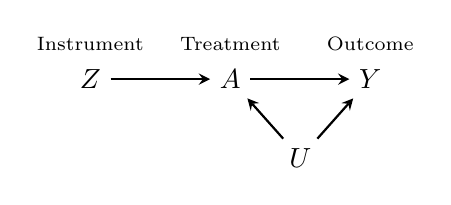
\begin{tikzpicture}[x = .7in]
    \node (z) at (-1,0) {$Z$};
    \node (a) at (0,0) {$A$};
    \node (y) at  (1,0) {$Y$};
    \node (u) at  (.5,-1) {$U$};
    \node[font = \scriptsize, anchor = south] at (z.north) {Instrument};
    \node[font = \scriptsize, anchor = south] at (a.north) {Treatment};
    \node[font = \scriptsize, anchor = south] at (y.north) {Outcome};
    \draw[->, >=stealth, thick] (z) -- (a);
    \draw[->, >=stealth, thick] (a) --  (y);
    \draw[->, >=stealth, thick] (u) --  (a);
    \draw[->, >=stealth, thick] (u) --  (y);
   \end{tikzpicture}
   \end{center}
\end{frame}}

\title{Instrumental variables}
\author{Soc 212C}
\date{Spring 2025}

\begin{document}

\maketitle

\begin{frame}{Instrumental variables}
A popular approach to causal inference with unmeasured treatment-outcome confounding \vskip .2in
We will discuss
\begin{itemize}
\item IV in randomized experiments with non-compliance
\item IV in observational settings
\end{itemize} \vskip .2in
Like all methods for causal inference from observational data,\\IV requires untestable assumptions that may be doubtful in many applications
\end{frame}

\begin{frame}[t]{Instrumental variables: Experiment with noncompliance} \vskip .25in
\begin{center}
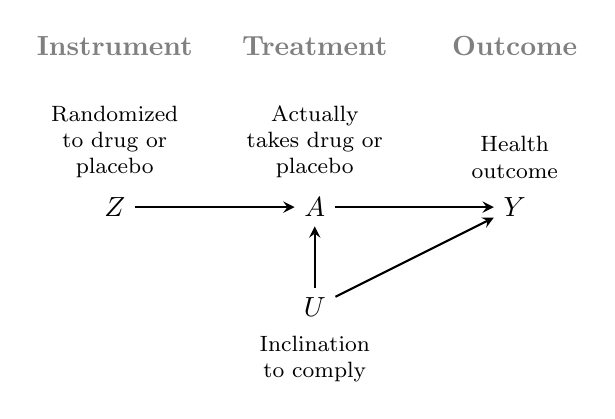
\begin{tikzpicture}[x = 1in, y = .5in]
    \node (z) at (-1,0) {$Z$};
    \node (a) at (0,0)   {$A$};
    \node (y) at  (1,0) {$Y$};
    \node (u) at  (0,-1) {$U$};
    \draw[->, >=stealth, thick] (z) -- (a);
    \draw[->, >=stealth, thick] (a) --  (y);
    \draw[->, >=stealth, thick] (u) --  (a);
    \draw[->, >=stealth, thick] (u) --  (y);
    \node[anchor = south, align = center, font = \footnotesize] at (z.north) {Randomized\\to drug or\\placebo};
    \node[anchor = south, align = center, font = \footnotesize] at (a.north) {Actually\\takes drug or\\placebo};
    \node[anchor = south, align = center, font = \footnotesize] at (y.north) {Health\\outcome};
    \node[anchor = north, align = center, font = \footnotesize] at (u.south) {Inclination\\to comply};
    \onslide<2->{
    	\node[anchor = north, font = \bf, gray] at (-1,1.8) {Instrument};
    	\node[anchor = north, font = \bf, gray] at (0,1.8) {Treatment};
    	\node[anchor = north, font = \bf, gray] at (1,1.8) {Outcome};
    }
  \end{tikzpicture}
\end{center}
\onslide<3->{
Two ideas
\begin{enumerate}
\item Intent to treat effect
\item Average effect among compliers
\end{enumerate}
}
\end{frame}

\begin{frame}[t]{Instrumental variables: 1) Intent to treat effect} \vskip .1in
\begin{center}
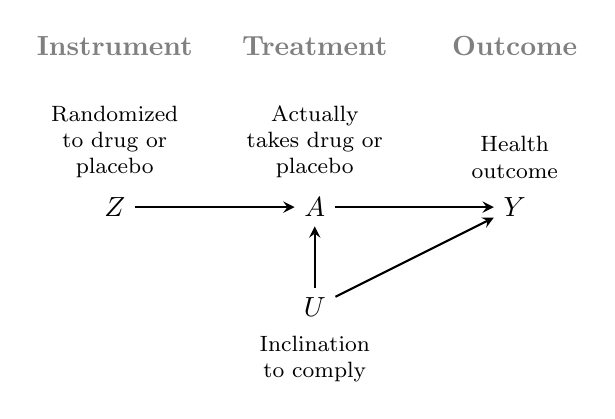
\begin{tikzpicture}[x = 1in, y = .5in]
    \node (z) at (-1,0) {$Z$};
    \node (a) at (0,0) {$A$};
    \node (y) at  (1,0) {$Y$};
    \node (u) at  (0,-1) {$U$};
    \draw[->, >=stealth, thick] (z) -- (a);
    \draw[->, >=stealth, thick] (a) --  (y);
    \draw[->, >=stealth, thick] (u) --  (a);
    \draw[->, >=stealth, thick] (u) --  (y);
    \node[anchor = south, align = center, font = \footnotesize] at (z.north) {Randomized\\to drug or\\placebo};
    \node[anchor = south, align = center, font = \footnotesize] at (a.north) {Actually\\takes drug or\\placebo};
    \node[anchor = south, align = center, font = \footnotesize] at (y.north) {Health\\outcome};
    \node[anchor = north, align = center, font = \footnotesize] at (u.south) {Inclination\\to comply};
    \node[anchor = north, font = \bf, gray] at (-1,1.8) {Instrument};
    \node[anchor = north, font = \bf, gray] at (0,1.8) {Treatment};
    \node[anchor = north, font = \bf, gray] at (1,1.8) {Outcome};
  \end{tikzpicture}
\end{center} \pause
Ignore $A$. What is the effect of $Z$ on $Y$?
\begin{center}
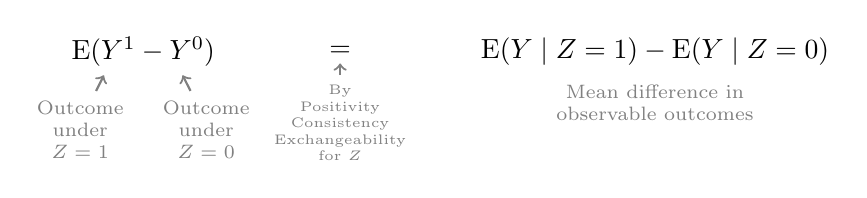
\begin{tikzpicture} \pause
\node at (-2.5,0) {$\E(Y^1 - Y^0)$};
\node[anchor = north, font = \scriptsize, gray, align = center] at (-3.3,-.5) {Outcome\\under\\$Z = 1$};
\node[anchor = north, font = \scriptsize, gray, align = center] at (-1.7,-.5) {Outcome\\under\\$Z = 0$};
\draw[->, thick, gray] (-3.1,-.5) -- (-3,-.3);
\draw[->, thick, gray] (-1.9,-.5) -- (-2,-.3);
\pause
\node at (0,0) {$=$};
\node[anchor = north, font = \tiny, gray, align = center] at (0,-.3) {By\\Positivity\\Consistency\\Exchangeability\\for $Z$};
\draw[->, thick, gray] (0,-.3) -- (0,-.15);
\pause
\node at (4,0) {$\E(Y\mid Z = 1) - \E(Y\mid Z = 0)$};
\node[anchor = north, font = \scriptsize, gray, align = center] at (4,-.3) {Mean difference in\\observable outcomes};
\end{tikzpicture}
\end{center}
\end{frame}

\begin{frame}[t]{Instrumental variables: 2) Average effect among compliers} \vskip .5in
Imbens, G., \& Angrist, J. (1994). \bref{https://www.nber.org/papers/t0118}{Identification and estimation of local average treatment effects.} Econometrica, 62(2), 467-475.
\end{frame}

\begin{frame}[t]{Instrumental variables: 2) Average effect among compliers} \vskip .1in
\begin{center}
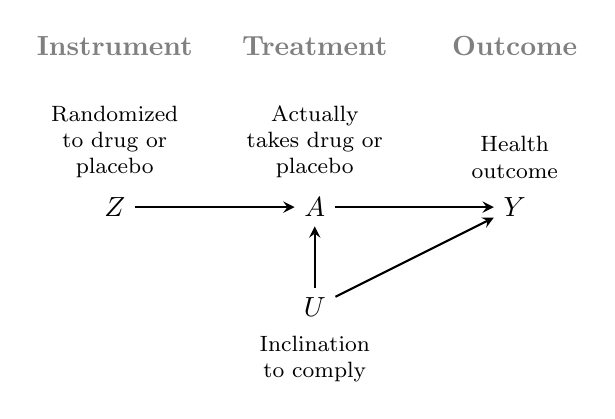
\begin{tikzpicture}[x = 1in, y = .5in]
    \node (z) at (-1,0) {$Z$};
    \node (a) at (0,0) {$A$};
    \node (y) at  (1,0) {$Y$};
    \node (u) at  (0,-1) {$U$};
    \draw[->, >=stealth, thick] (z) -- (a);
    \draw[->, >=stealth, thick] (a) --  (y);
    \draw[->, >=stealth, thick] (u) --  (a);
    \draw[->, >=stealth, thick] (u) --  (y);
    \node[anchor = south, align = center, font = \footnotesize] at (z.north) {Randomized\\to drug or\\placebo};
    \node[anchor = south, align = center, font = \footnotesize] at (a.north) {Actually\\takes drug or\\placebo};
    \node[anchor = south, align = center, font = \footnotesize] at (y.north) {Health\\outcome};
    \node[anchor = north, align = center, font = \footnotesize] at (u.south) {Inclination\\to comply};
    \node[anchor = north, font = \bf, gray] at (-1,1.8) {Instrument};
    \node[anchor = north, font = \bf, gray] at (0,1.8) {Treatment};
    \node[anchor = north, font = \bf, gray] at (1,1.8) {Outcome};
  \end{tikzpicture}
\end{center} \pause
\bblue{Key insight}: The effect of $Z$ on $Y$ operates entirely through $A$
\begin{enumerate} \pause
\item Study the effect of $Z\rightarrow Y$ \hfill \pause (we just did) \pause
\item Study the effect of $Z\rightarrow A$ \pause
\item Learn about $A \rightarrow Y$ since $Z\rightarrow Y$ is $Z\rightarrow A \rightarrow Y$
\end{enumerate}
\end{frame}

\begin{frame}[t]{Instrumental variables: 2) Average effect among compliers} \vskip .1in
\begin{center}
\scalebox{.4}{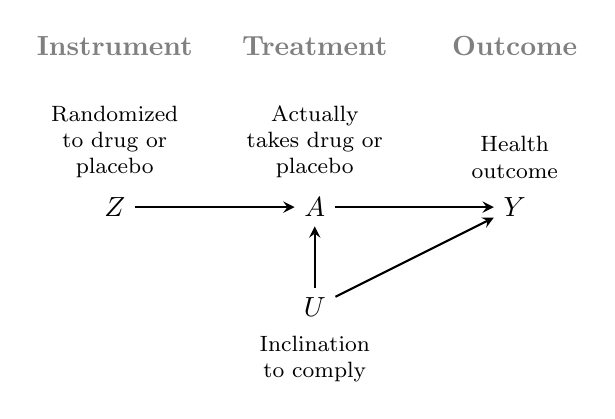
\begin{tikzpicture}[x = 1in, y = .5in]
    \node (z) at (-1,0) {$Z$};
    \node (a) at (0,0) {$A$};
    \node (y) at  (1,0) {$Y$};
    \node (u) at  (0,-1) {$U$};
    \draw[->, >=stealth, thick] (z) -- (a);
    \draw[->, >=stealth, thick] (a) --  (y);
    \draw[->, >=stealth, thick] (u) --  (a);
    \draw[->, >=stealth, thick] (u) --  (y);
    \node[anchor = south, align = center, font = \footnotesize] at (z.north) {Randomized\\to drug or\\placebo};
    \node[anchor = south, align = center, font = \footnotesize] at (a.north) {Actually\\takes drug or\\placebo};
    \node[anchor = south, align = center, font = \footnotesize] at (y.north) {Health\\outcome};
    \node[anchor = north, align = center, font = \footnotesize] at (u.south) {Inclination\\to comply};
    \node[anchor = north, font = \bf, gray] at (-1,1.8) {Instrument};
    \node[anchor = north, font = \bf, gray] at (0,1.8) {Treatment};
    \node[anchor = north, font = \bf, gray] at (1,1.8) {Outcome};
  \end{tikzpicture}}
\end{center} \pause
The effect $Z\rightarrow A$ has four \bblue{principal strata}:\\latent sets of people who respond to $Z$ a particular way \pause
$$\begin{aligned}
\text{Compliers}\qquad & A^{Z=0} = 0 & A^{Z=1} = 1&\qquad\text{(follow assignment)} \\ \pause
\text{Always takers}\qquad & A^{Z=0} = 1 & A^{Z=1} = 1&\qquad\text{(always take treatment)} \\ \pause
\text{Never takers}\qquad & A^{Z=0} = 0 & A^{Z=1} = 0&\qquad\text{(never take treatment)} \\ \pause
\text{Defiers}\qquad & A^{Z=0} = 1 & A^{Z=1} = 0 &\qquad\text{(defy assignment)}
\end{aligned}$$ \pause
\bgray{Discuss:} In which strata is the effect $Z\rightarrow Y$ zero?
\end{frame}

\begin{frame}[t]{Instrumental variables: 2) Average effect among compliers} \vskip .1in
\begin{center}
\scalebox{.4}{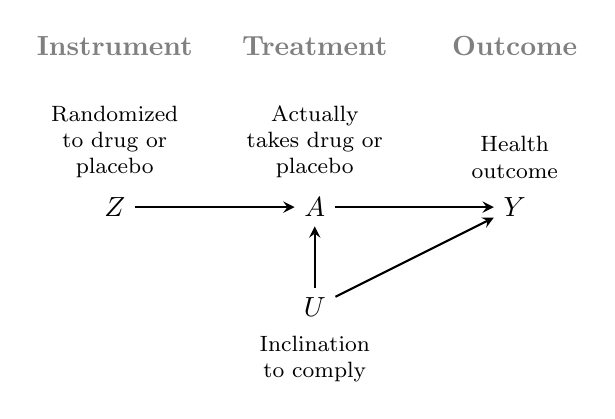
\begin{tikzpicture}[x = 1in, y = .5in]
    \node (z) at (-1,0) {$Z$};
    \node (a) at (0,0) {$A$};
    \node (y) at  (1,0) {$Y$};
    \node (u) at  (0,-1) {$U$};
    \draw[->, >=stealth, thick] (z) -- (a);
    \draw[->, >=stealth, thick] (a) --  (y);
    \draw[->, >=stealth, thick] (u) --  (a);
    \draw[->, >=stealth, thick] (u) --  (y);
    \node[anchor = south, align = center, font = \footnotesize] at (z.north) {Randomized\\to drug or\\placebo};
    \node[anchor = south, align = center, font = \footnotesize] at (a.north) {Actually\\takes drug or\\placebo};
    \node[anchor = south, align = center, font = \footnotesize] at (y.north) {Health\\outcome};
    \node[anchor = north, align = center, font = \footnotesize] at (u.south) {Inclination\\to comply};
    \node[anchor = north, font = \bf, gray] at (-1,1.8) {Instrument};
    \node[anchor = north, font = \bf, gray] at (0,1.8) {Treatment};
    \node[anchor = north, font = \bf, gray] at (1,1.8) {Outcome};
  \end{tikzpicture}}
\end{center}
Among \bgray{always takers} and \bgray{never takers},\\ \pause
$Z$ does not affect $A$ \pause \vskip .1in
$Z$ only affects $Y$ through $A$ \pause \vskip .1in
In these strata, $Z$ does not affect $Y$
\end{frame}

\begin{frame}[t]{Instrumental variables: 2) Average effect among compliers} \vskip .1in
\begin{center}
\scalebox{.4}{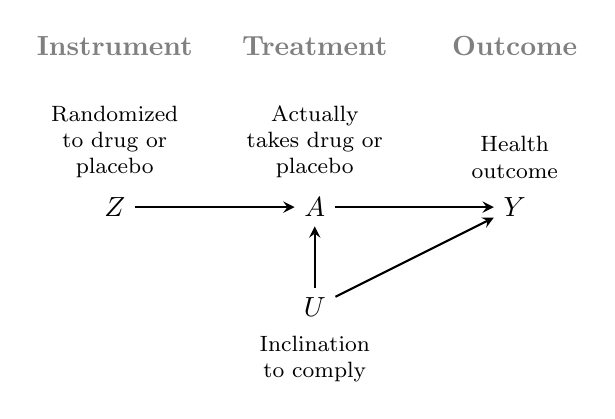
\begin{tikzpicture}[x = 1in, y = .5in]
    \node (z) at (-1,0) {$Z$};
    \node (a) at (0,0) {$A$};
    \node (y) at  (1,0) {$Y$};
    \node (u) at  (0,-1) {$U$};
    \draw[->, >=stealth, thick] (z) -- (a);
    \draw[->, >=stealth, thick] (a) --  (y);
    \draw[->, >=stealth, thick] (u) --  (a);
    \draw[->, >=stealth, thick] (u) --  (y);
    \node[anchor = south, align = center, font = \footnotesize] at (z.north) {Randomized\\to drug or\\placebo};
    \node[anchor = south, align = center, font = \footnotesize] at (a.north) {Actually\\takes drug or\\placebo};
    \node[anchor = south, align = center, font = \footnotesize] at (y.north) {Health\\outcome};
    \node[anchor = north, align = center, font = \footnotesize] at (u.south) {Inclination\\to comply};
    \node[anchor = north, font = \bf, gray] at (-1,1.8) {Instrument};
    \node[anchor = north, font = \bf, gray] at (0,1.8) {Treatment};
    \node[anchor = north, font = \bf, gray] at (1,1.8) {Outcome};
  \end{tikzpicture}}
\end{center}
Among \bgray{compliers}, \pause \\
$Z = 1$ implies $A = 1$ and\\$Z = 0$ implies $A = 0$ \pause \vskip .1in
In these strata, $Z = A$ \pause \vskip .1in
$Z\rightarrow Y$ and $A\rightarrow Y$ are the same
\end{frame}

\begin{frame}[t]{Instrumental variables: 2) Average effect among compliers} \vskip .1in
\begin{center}
\scalebox{.4}{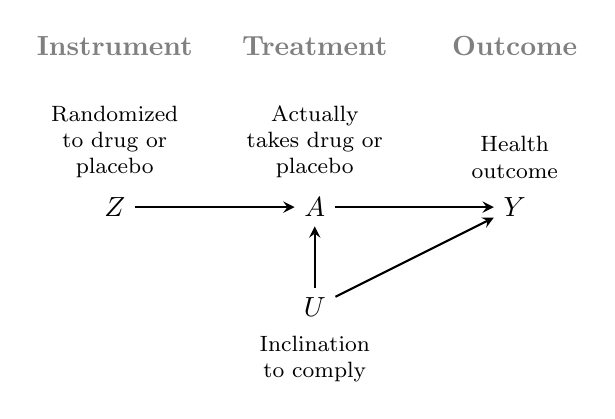
\begin{tikzpicture}[x = 1in, y = .5in]
    \node (z) at (-1,0) {$Z$};
    \node (a) at (0,0) {$A$};
    \node (y) at  (1,0) {$Y$};
    \node (u) at  (0,-1) {$U$};
    \draw[->, >=stealth, thick] (z) -- (a);
    \draw[->, >=stealth, thick] (a) --  (y);
    \draw[->, >=stealth, thick] (u) --  (a);
    \draw[->, >=stealth, thick] (u) --  (y);
    \node[anchor = south, align = center, font = \footnotesize] at (z.north) {Randomized\\to drug or\\placebo};
    \node[anchor = south, align = center, font = \footnotesize] at (a.north) {Actually\\takes drug or\\placebo};
    \node[anchor = south, align = center, font = \footnotesize] at (y.north) {Health\\outcome};
    \node[anchor = north, align = center, font = \footnotesize] at (u.south) {Inclination\\to comply};
    \node[anchor = north, font = \bf, gray] at (-1,1.8) {Instrument};
    \node[anchor = north, font = \bf, gray] at (0,1.8) {Treatment};
    \node[anchor = north, font = \bf, gray] at (1,1.8) {Outcome};
  \end{tikzpicture}}
\end{center}
Among \bgray{defiers}, \pause \\
$Z = 1$ implies $A = 0$ and\\$Z = 0$ implies $A = 1$ \pause \vskip .1in
In these strata, $Z = 1-A$ \pause \vskip .1in
$Z\rightarrow Y$ and $A\rightarrow Y$ are the same magnitude\\but have opposite signs
\end{frame}

\begin{frame}[t]{Instrumental variables: 2) Average effect among compliers} \vskip .1in
\begin{center}
\scalebox{.4}{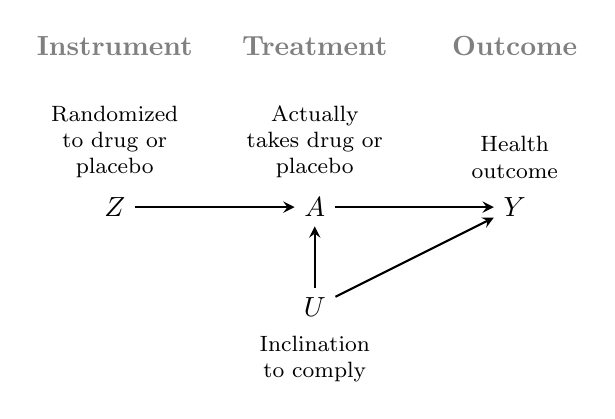
\begin{tikzpicture}[x = 1in, y = .5in]
    \node (z) at (-1,0) {$Z$};
    \node (a) at (0,0) {$A$};
    \node (y) at  (1,0) {$Y$};
    \node (u) at  (0,-1) {$U$};
    \draw[->, >=stealth, thick] (z) -- (a);
    \draw[->, >=stealth, thick] (a) --  (y);
    \draw[->, >=stealth, thick] (u) --  (a);
    \draw[->, >=stealth, thick] (u) --  (y);
    \node[anchor = south, align = center, font = \footnotesize] at (z.north) {Randomized\\to drug or\\placebo};
    \node[anchor = south, align = center, font = \footnotesize] at (a.north) {Actually\\takes drug or\\placebo};
    \node[anchor = south, align = center, font = \footnotesize] at (y.north) {Health\\outcome};
    \node[anchor = north, align = center, font = \footnotesize] at (u.south) {Inclination\\to comply};
    \node[anchor = north, font = \bf, gray] at (-1,1.8) {Instrument};
    \node[anchor = north, font = \bf, gray] at (0,1.8) {Treatment};
    \node[anchor = north, font = \bf, gray] at (1,1.8) {Outcome};
  \end{tikzpicture}}
\end{center}
Four principal strata
$$\begin{aligned}
\text{Compliers} \qquad& (Z\rightarrow A) = +1\quad&& (Z\rightarrow Y) = (A\rightarrow Y)\phantom{-} \\
\text{Always takers} \qquad& (Z\rightarrow A) = 0&& (Z\rightarrow Y) = 0 \\
\text{Never takers} \qquad& (Z\rightarrow A) = 0&& (Z\rightarrow Y) = 0 \only<1-2>{\\}
\only<1>{\text{Defiers} \qquad& (Z\rightarrow A) = -1&& (Z\rightarrow Y) = -(A\rightarrow Y)}
\only<2>{\gray{\text{Defiers}} \qquad& \gray{(Z\rightarrow A) = -1}&& \gray{(Z\rightarrow Y) = -(A\rightarrow Y)}}
\end{aligned}$$
\only<2>{Assume \bblue{no defiers} in the population}

\onslide<4->{\bgray{Discuss a hypothetical.}}\\
\onslide<5->{Population is 50\% compliers, 25\% always takers, 25\% never takers}\\
\onslide<6->{Average effect of $Z\rightarrow Y$ among compliers is 0.6}\vskip .1in
\onslide<7->{What is the average effect of $Z\rightarrow Y$ in the population? \only<8->{\bblue{0.3}}}

\end{frame}

\begin{frame}{Instrumental variables: 2) Average effect among compliers}
Deriving the general case: \pause
$$\begin{small}
\begin{aligned}
&\E(Y^{Z = 1} - Y^{Z = 0}) \\ \pause
&= \sum_s \E(Y^{Z = 1} - Y^{Z = 0}\mid S = s)\underbrace{\P(S = s)}_{\substack{\text{Denote}\\\pi_s}} \\ \pause
&= \E(Y^{Z = 1} - Y^{Z = 0}\mid S = \text{Complier})\pi_\text{Complier} \\
&\qquad + \E(Y^{Z = 1} - Y^{Z = 0}\mid S = \text{Always-Taker})\pi_\text{Always-Taker} &\onslide<5->{\gray{(=0)}} \\
&\qquad + \E(Y^{Z = 1} - Y^{Z = 0}\mid S = \text{Never-Taker})\pi_\text{Never-Taker}  &\onslide<5->{\gray{(=0)}}\\
&\qquad + \E(Y^{Z = 1} - Y^{Z = 0}\mid S = \text{Defier})\pi_\text{Defier} &\onslide<5->{\gray{(=0)}}
\end{aligned}
\end{small}$$

\end{frame}


\begin{frame}{Instrumental variables: 2) Average effect among compliers}
\begin{center}
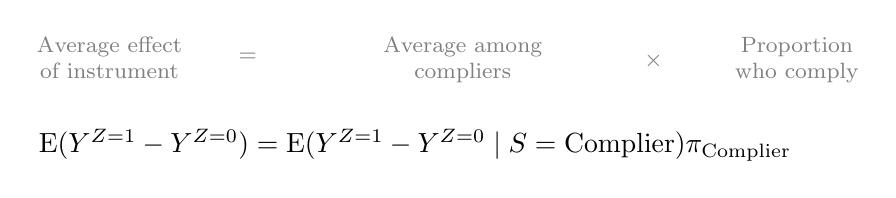
\begin{tikzpicture}[x = .5\textwidth]
\node at (0,0) {$\E(Y^{Z = 1} - Y^{Z = 0}) = \E(Y^{Z = 1} - Y^{Z = 0}\mid S = \text{Complier})\pi_\text{Complier}$}; \pause
\node[anchor = north, font = \footnotesize, gray, align = center] at (-.64,1.5) {Average effect\\of instrument};
\node[anchor = north, font = \footnotesize, gray, align = center] at (-.35,1.3) {=};
\node[anchor = north, font = \footnotesize, gray, align = center] at (.1,1.5) {Average among\\compliers};
\node[anchor = north, font = \footnotesize, gray, align = center] at (.5,1.3) {$\times$};
\node[anchor = north, font = \footnotesize, gray, align = center] at (.8,1.5) {Proportion\\who comply};
\end{tikzpicture}
\end{center} \onslide<3->{
Among compliers, ($Z\rightarrow Y$) = ($A\rightarrow Y$).
}
\onslide<4->{
$$\E(Y^{Z = 1} - Y^{Z = 0}) = \E(Y^{A = 1} - Y^{A = 0}\mid S = \text{Complier})\pi_\text{Complier}$$
}
\onslide<5->{
Rearrange to get the complier average treatment effect
}
\onslide<6->{$$\begin{aligned}
\E(Y^{A = 1} - Y^{A = 0}\mid S = \text{Complier}) &= \frac{\E(Y^{Z = 1} - Y^{Z = 0})}{\pi_\text{Complier}} \\
}
\onslide<7->{
&= \frac{\E(Y^{Z = 1} - Y^{Z = 0})}{\E(A^{Z = 1} - A^{Z = 0})}
\end{aligned}$$
}
\end{frame}

\begin{frame}

\huge
IV in observational settings

\end{frame}

\begin{frame}{Running example}
\centering
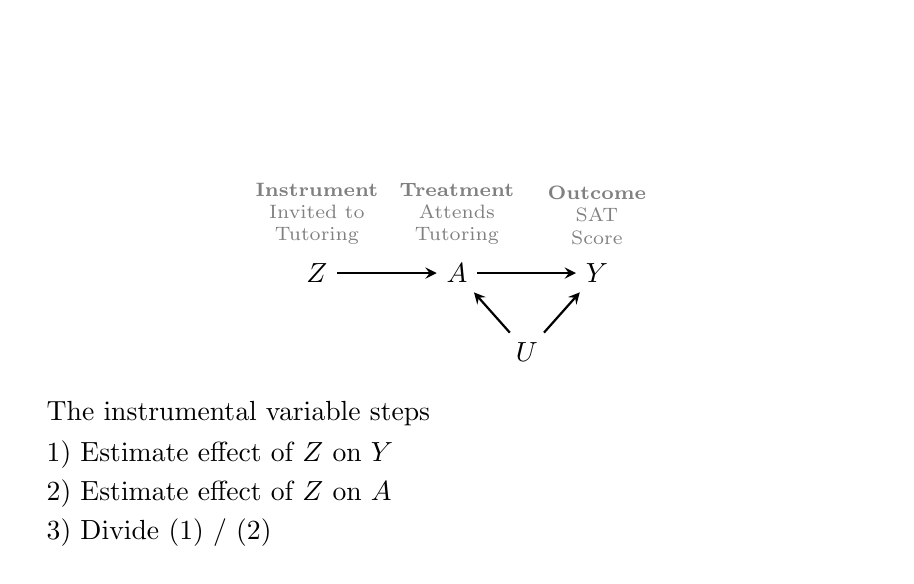
\begin{tikzpicture}[x = .7in]
    \node at (-3,-3) {};
    \node at (3,3) {};
    \node (z) at (-1,0) {$Z$};
    \node (a) at (0,0) {$A$};
    \node (y) at  (1,0) {$Y$};
    \node (u) at  (.5,-1) {$U$};
    \node[font = \scriptsize, anchor = south, align = center, gray] at (z.north) {\textbf{Instrument}\\Invited to\\Tutoring};
    \node[font = \scriptsize, anchor = south, align = center, gray] at (a.north) {\textbf{Treatment}\\Attends\\Tutoring};
    \node[font = \scriptsize, anchor = south, align = center, gray] at (y.north) {\textbf{Outcome}\\SAT\\Score};
    \draw[->, >=stealth, thick] (z) -- (a);
    \draw[->, >=stealth, thick] (a) --  (y);
    \draw[->, >=stealth, thick] (u) --  (a);
    \draw[->, >=stealth, thick] (u) --  (y);
    \node[anchor = north west] at (-3,-1.5) {The instrumental variable steps};
    \node[anchor = north west] at (-3,-2) {1) Estimate effect of $Z$ on $Y$};
    \node[anchor = north west] at (-3,-2.5) {2) Estimate effect of $Z$ on $A$};
    \node[anchor = north west] at (-3,-3) {3) Divide (1) / (2)};
   \end{tikzpicture}
\end{frame}

\begin{frame}{Requirement 1) Instrument exchangeability}
\centering
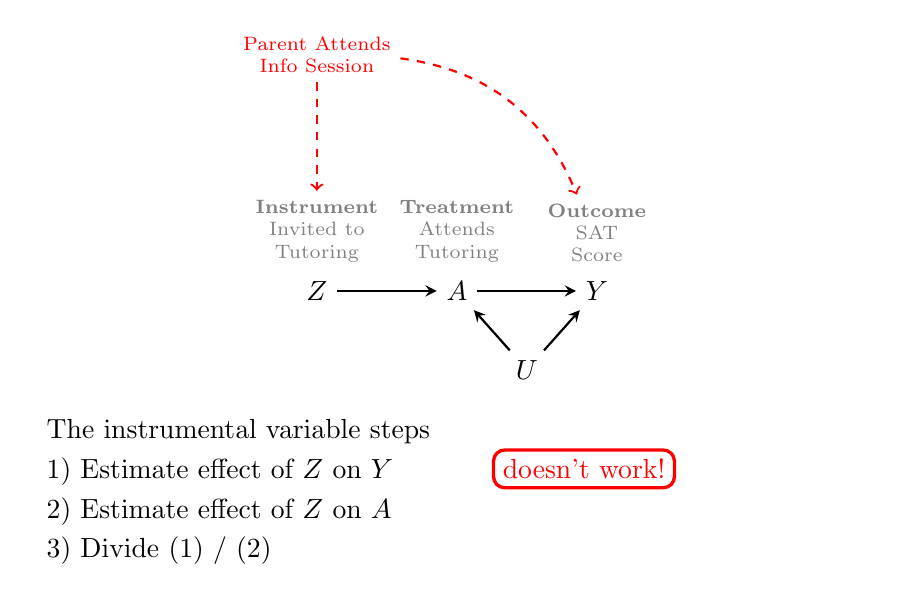
\begin{tikzpicture}[x = .7in]
\node at (-3,-3) {};
\node at (3,3) {};
    \node (z) at (-1,0) {$Z$};
    \node (a) at (0,0) {$A$};
    \node (y) at  (1,0) {$Y$};
    \node (u) at  (.5,-1) {$U$};
    \node[font = \scriptsize, anchor = south, align = center, gray] (zlab) at (z.north) {\textbf{Instrument}\\Invited to\\Tutoring};
    \node[font = \scriptsize, anchor = south, align = center, gray] (alab) at (a.north) {\textbf{Treatment}\\Attends\\Tutoring};
    \node[font = \scriptsize, anchor = south, align = center, gray] (ylab) at (y.north) {\textbf{Outcome}\\SAT\\Score};
    \draw[->, >=stealth, thick] (z) -- (a);
    \draw[->, >=stealth, thick] (a) --  (y);
    \draw[->, >=stealth, thick] (u) --  (a);
    \draw[->, >=stealth, thick] (u) --  (y);
    \node[anchor = north west] at (-3,-1.5) {The instrumental variable steps};
    \node[anchor = north west] at (-3,-2) {1) Estimate effect of $Z$ on $Y$};
    \node[anchor = north west] at (-3,-2.5) {2) Estimate effect of $Z$ on $A$};
    \node[anchor = north west] at (-3,-3) {3) Divide (1) / (2)};
    \pause
    \node[font = \scriptsize, align = center, red] (v) at (-1,3) {Parent Attends\\Info Session};
    \draw[->, thick, red, dashed] (v) -- (zlab);
    \pause
    \draw[->, thick, red, dashed] (v) to[bend left] (ylab);
    \pause
    \node[anchor = north west, font = \red, draw = red, line width = 1.2pt, rounded corners] at (.25,-2) {doesn't work!};
   \end{tikzpicture}
\end{frame}

\begin{frame}{Requirement 2) No direct effect of $Z$ on $Y$}
\centering
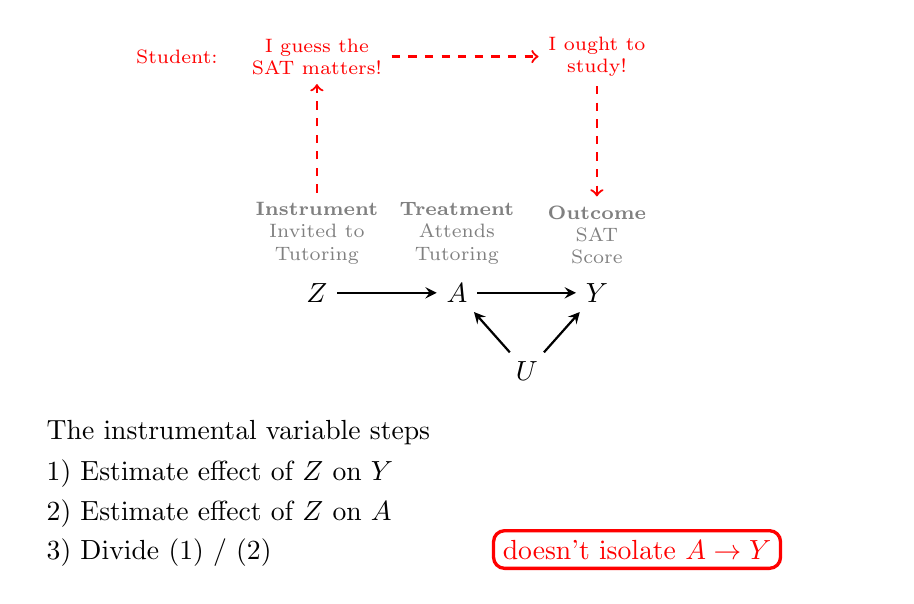
\begin{tikzpicture}[x = .7in]
\node at (-3,-3) {};
\node at (3,3) {};
    \node (z) at (-1,0) {$Z$};
    \node (a) at (0,0) {$A$};
    \node (y) at  (1,0) {$Y$};
    \node (u) at  (.5,-1) {$U$};
    \node[font = \scriptsize, anchor = south, align = center, gray] (zlab) at (z.north) {\textbf{Instrument}\\Invited to\\Tutoring};
    \node[font = \scriptsize, anchor = south, align = center, gray] (alab) at (a.north) {\textbf{Treatment}\\Attends\\Tutoring};
    \node[font = \scriptsize, anchor = south, align = center, gray] (ylab) at (y.north) {\textbf{Outcome}\\SAT\\Score};
    \draw[->, >=stealth, thick] (z) -- (a);
    \draw[->, >=stealth, thick] (a) --  (y);
    \draw[->, >=stealth, thick] (u) --  (a);
    \draw[->, >=stealth, thick] (u) --  (y);
    \node[anchor = north west] at (-3,-1.5) {The instrumental variable steps};
    \node[anchor = north west] (one) at (-3,-2) {1) Estimate effect of $Z$ on $Y$};
    \node[anchor = north west] (two) at (-3,-2.5) {2) Estimate effect of $Z$ on $A$};
    \node[anchor = north west] (three) at (-3,-3) {3) Divide (1) / (2)};
    \pause
    \node[font = \scriptsize, align = center, red] at (-2,3) {Student:};
    \node[font = \scriptsize, align = center, red] (v) at (-1,3) {I guess the\\SAT matters!};
    \draw[->, thick, red, dashed] (zlab) -- (v);
    \pause
    \node[font = \scriptsize, align = center, red] (v2) at (1,3) {I ought to\\study!};
    \draw[->, thick, red, dashed] (v) -- (v2);
    \pause
    \draw[->, thick, red, dashed] (v2) -- (ylab);
    \pause
    \node[anchor = north west, font = \red, draw = red, line width = 1.2pt, rounded corners] at (.25,-3) {doesn't isolate $A\rightarrow Y$};
   \end{tikzpicture}
\end{frame}


\begin{frame}{Requirement 3) Relevance}
\centering
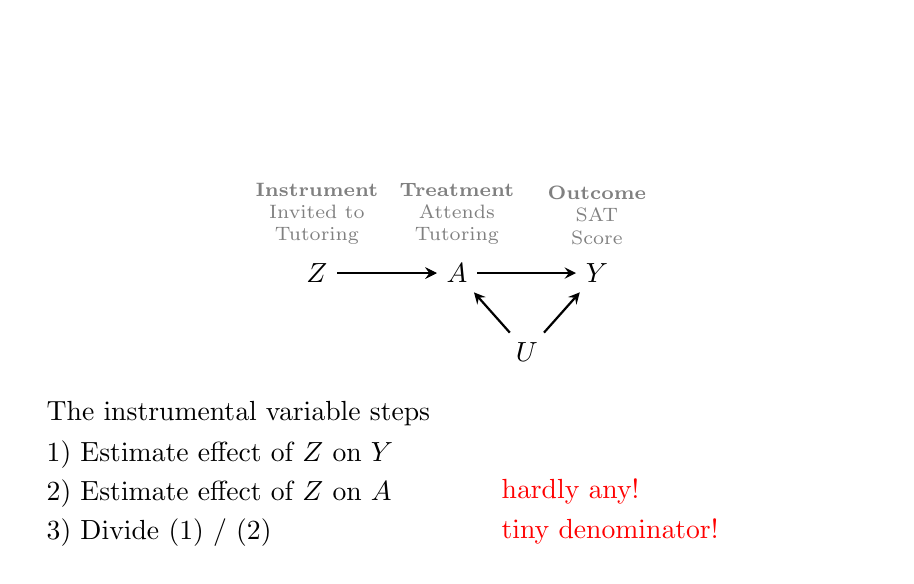
\begin{tikzpicture}[x = .7in]
\node at (-3,-3) {};
\node at (3,3) {};
    \node (z) at (-1,0) {$Z$};
    \node (a) at (0,0) {$A$};
    \node (y) at  (1,0) {$Y$};
    \node (u) at  (.5,-1) {$U$};
    \node[font = \scriptsize, anchor = south, align = center, gray] (zlab) at (z.north) {\textbf{Instrument}\\Invited to\\Tutoring};
    \node[font = \scriptsize, anchor = south, align = center, gray] (alab) at (a.north) {\textbf{Treatment}\\Attends\\Tutoring};
    \node[font = \scriptsize, anchor = south, align = center, gray] (ylab) at (y.north) {\textbf{Outcome}\\SAT\\Score};
    \draw<1>[->, >=stealth, thick] (z) -- (a);
    \draw<2->[->, >=stealth, thick, dotted] (z) -- (a);
    \draw[->, >=stealth, thick] (a) --  (y);
    \draw[->, >=stealth, thick] (u) --  (a);
    \draw[->, >=stealth, thick] (u) --  (y);
    \node[anchor = north west] at (-3,-1.5) {The instrumental variable steps};
    \node[anchor = north west] (one) at (-3,-2) {1) Estimate effect of $Z$ on $Y$};
    \node[anchor = north west] (two) at (-3,-2.5) {2) Estimate effect of $Z$ on $A$};
    \node[anchor = north west] (three) at (-3,-3) {3) Divide (1) / (2)};
    \pause
    \node[anchor = north west, font = \red] at (.25,-2.5) {hardly any!};
    \pause
    \node[anchor = north west, font = \red] at (.25,-3) {tiny denominator!};
   \end{tikzpicture}
\end{frame}

\begin{frame}{Requirement 4a) Homogeneity}
\centering
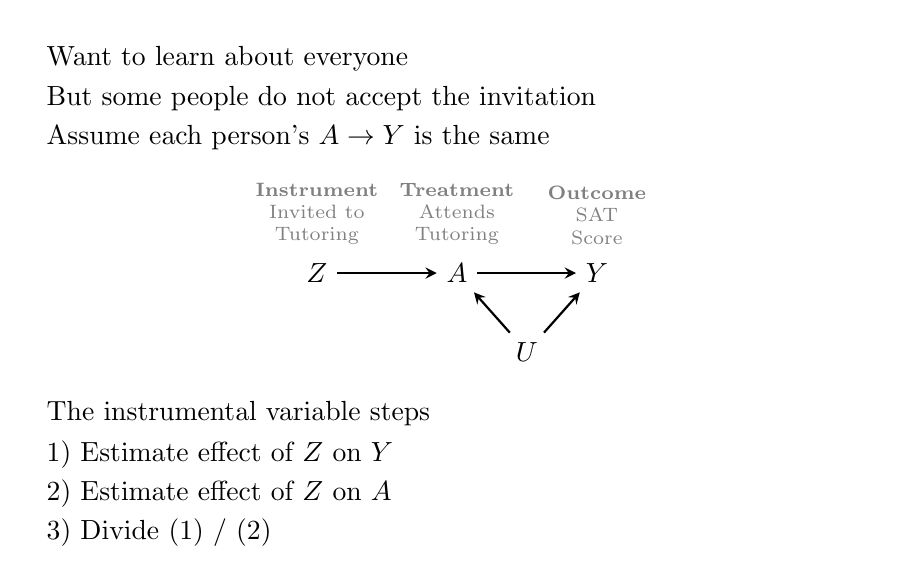
\begin{tikzpicture}[x = .7in]
\node at (-3,-3) {};
\node at (3,3) {};
    \node (z) at (-1,0) {$Z$};
    \node (a) at (0,0) {$A$};
    \node (y) at  (1,0) {$Y$};
    \node (u) at  (.5,-1) {$U$};
    \node[font = \scriptsize, anchor = south, align = center, gray] (zlab) at (z.north) {\textbf{Instrument}\\Invited to\\Tutoring};
    \node[font = \scriptsize, anchor = south, align = center, gray] (alab) at (a.north) {\textbf{Treatment}\\Attends\\Tutoring};
    \node[font = \scriptsize, anchor = south, align = center, gray] (ylab) at (y.north) {\textbf{Outcome}\\SAT\\Score};
    \draw[->, >=stealth, thick] (z) -- (a);
    \draw[->, >=stealth, thick] (a) --  (y);
    \draw[->, >=stealth, thick] (u) --  (a);
    \draw[->, >=stealth, thick] (u) --  (y);
    \node[anchor = north west] at (-3,-1.5) {The instrumental variable steps};
    \node[anchor = north west] (one) at (-3,-2) {1) Estimate effect of $Z$ on $Y$};
    \node[anchor = north west] (two) at (-3,-2.5) {2) Estimate effect of $Z$ on $A$};
    \node[anchor = north west] (three) at (-3,-3) {3) Divide (1) / (2)};
    \pause
    \node[anchor = north west] at (-3,3) {Want to learn about everyone};
    \pause
    \node[anchor = north west] at (-3,2.5) {But some people do not accept the invitation};
    \pause
    \node[anchor = north west] at (-3,2) {Assume each person's $A\rightarrow Y$ is the same};
   \end{tikzpicture}
\end{frame}

\begin{frame}{Requirement 4b) Monotonicity}
\centering
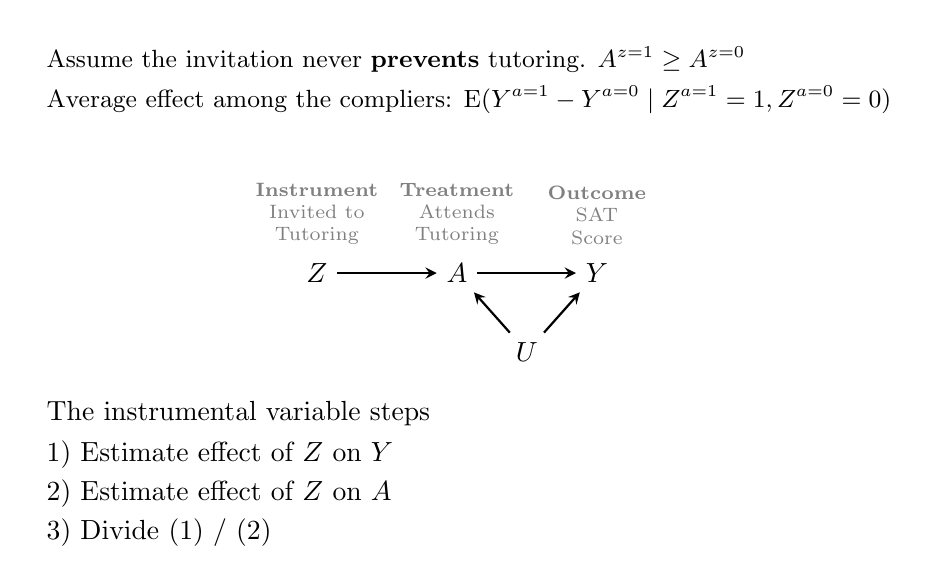
\begin{tikzpicture}[x = .7in]
\node at (-3,-3) {};
\node at (3,3) {};
    \node (z) at (-1,0) {$Z$};
    \node (a) at (0,0) {$A$};
    \node (y) at  (1,0) {$Y$};
    \node (u) at  (.5,-1) {$U$};
    \node[font = \scriptsize, anchor = south, align = center, gray] (zlab) at (z.north) {\textbf{Instrument}\\Invited to\\Tutoring};
    \node[font = \scriptsize, anchor = south, align = center, gray] (alab) at (a.north) {\textbf{Treatment}\\Attends\\Tutoring};
    \node[font = \scriptsize, anchor = south, align = center, gray] (ylab) at (y.north) {\textbf{Outcome}\\SAT\\Score};
    \draw[->, >=stealth, thick] (z) -- (a);
    \draw[->, >=stealth, thick] (a) --  (y);
    \draw[->, >=stealth, thick] (u) --  (a);
    \draw[->, >=stealth, thick] (u) --  (y);
    \node[anchor = north west] at (-3,-1.5) {The instrumental variable steps};
    \node[anchor = north west] (one) at (-3,-2) {1) Estimate effect of $Z$ on $Y$};
    \node[anchor = north west] (two) at (-3,-2.5) {2) Estimate effect of $Z$ on $A$};
    \node[anchor = north west] (three) at (-3,-3) {3) Divide (1) / (2)};
    \pause
    \node[anchor = north west, font = \small] at (-3,3) {Assume the invitation never \textbf{prevents} tutoring. $A^{z=1} \geq A^{z=0}$};
    \pause
    \node[anchor = north west, font = \small] at (-3,2.5) {Average effect among the compliers: $\E(Y^{a=1} - Y^{a=0}\mid Z^{a=1} = 1, Z^{a=0} = 0)$};
   \end{tikzpicture}
\end{frame}

\begin{frame}{IV requires (1--3) and either (4a) or (4b)}

\begin{itemize}
\item[1)] instrument exchangeability
\item[2)] no direct $Z\rightarrow Y$ effect
\item[3)] relevance so that $Z$ is related to $A$
\end{itemize} \vskip .1in
and either
\begin{itemize}
\item[4a)] homogeneity such that $A\rightarrow Y$ is constant, or
\item[4b)] monotonicity, such that $Z\rightarrow A$ is either\\positive for everyone or negative for everyone
\end{itemize}

\vskip .1in
\begin{center}
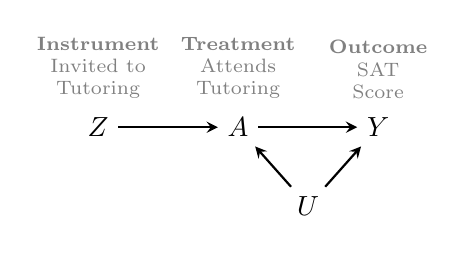
\begin{tikzpicture}[x = .7in]
    \node (z) at (-1,0) {$Z$};
    \node (a) at (0,0) {$A$};
    \node (y) at  (1,0) {$Y$};
    \node (u) at  (.5,-1) {$U$};
    \node[font = \scriptsize, anchor = south, align = center, gray] at (z.north) {\textbf{Instrument}\\Invited to\\Tutoring};
    \node[font = \scriptsize, anchor = south, align = center, gray] at (a.north) {\textbf{Treatment}\\Attends\\Tutoring};
    \node[font = \scriptsize, anchor = south, align = center, gray] at (y.north) {\textbf{Outcome}\\SAT\\Score};
    \draw[->, >=stealth, thick] (z) -- (a);
    \draw[->, >=stealth, thick] (a) --  (y);
    \draw[->, >=stealth, thick] (u) --  (a);
    \draw[->, >=stealth, thick] (u) --  (y);
   \end{tikzpicture}
 \end{center}

\end{frame}

\begin{frame}{Where to learn more}

Felton, C., and B.M. Stewart. 2024. \bref{https://doi.org/10.1177/00491241241235900}{``Handle with Care: A Sociologist’s Guide to Causal Inference with Instrumental Variables.''} Sociological Methods \& Research.

\end{frame}

\begin{frame}
\Large
An observational settings that is \bgray{clean}
\end{frame}

\begin{frame}

\includegraphics[height = .8\textheight]{figs/VietnamNumbers} \\
\url{https://www.historynet.com/whats-your-number/}

\end{frame}

\begin{frame}

\includegraphics[width = .6\textwidth]{figs/VietnamDraw}
\url{https://commons.wikimedia.org/wiki/File:1969_draft_lottery_photo.jpg}

\end{frame}

\begin{frame}%{Assumptions are less plausible in observational studies}

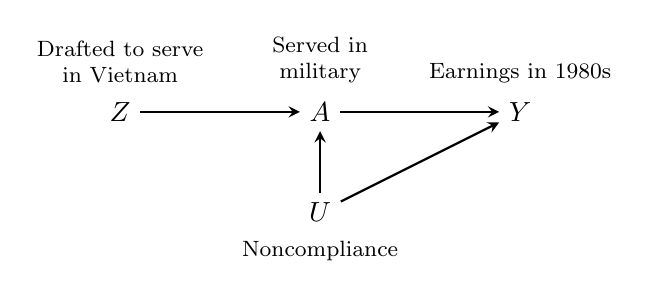
\begin{tikzpicture}[x = 1in, y = .5in]
    \node (z) at (-1,0) {$Z$};
    \node (a) at (0,0) {$A$};
    \node (y) at  (1,0) {$Y$};
    \node (u) at  (0,-1) {$U$};
    \draw[->, >=stealth, thick] (z) -- (a);
    \draw[->, >=stealth, thick] (a) --  (y);
    \draw[->, >=stealth, thick] (u) --  (a);
    \draw[->, >=stealth, thick] (u) --  (y);
    \node[anchor = south, align = center, font = \footnotesize] at (z.north) {Drafted to serve\\in Vietnam};
    \node[anchor = south, align = center, font = \footnotesize] at (a.north) {Served in\\military};
    \node[anchor = south, align = center, font = \footnotesize] at (y.north) {Earnings in 1980s};
    \node[anchor = north, align = center, font = \footnotesize] at (u.south) {Noncompliance};
    %\node[anchor = north, font = \bf, gray] at (-1,1.8) {Instrument};
    %\node[anchor = north, font = \bf, gray] at (0,1.8) {Treatment};
    %\node[anchor = north, font = \bf, gray] at (1,1.8) {Outcome};
  \end{tikzpicture} \vskip .1in \pause
  This is credible
  \begin{itemize} \pause
  \item Exogeneity: Randomly selected draft numbers \pause
  \item Exclusion: Being drafted affects earnings only through service \pause
  \item Monotonicity: No one joins the military in defiance of not being drafted
  \end{itemize}
   \vskip .2in
\begin{footnotesize}Angrist, J. D. (1990). \bref{https://www.jstor.org/stable/2006669}{Lifetime earnings and the Vietnam era draft lottery: Evidence from Social Security administrative records.} The American Economic Review, 313-336.
\end{footnotesize}

\end{frame}

\begin{frame}
\Large
Observational settings that are \bgray{less straightforward}
\end{frame}

\begin{frame}{A difficult example: Genes as instruments} \pause

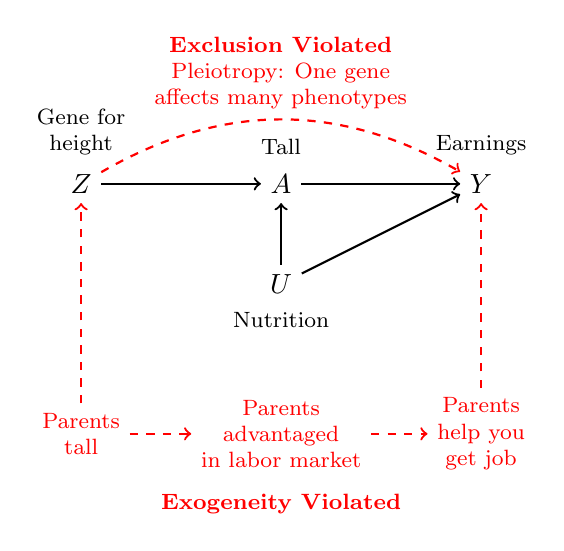
\begin{tikzpicture}[x = 1in, y = .5in]
    \node (z) at (-1,0) {$Z$};
    \node (a) at (0,0) {$A$};
    \node (y) at  (1,0) {$Y$};
    \node (u) at  (0,-1) {$U$};
    \node[anchor = south, align = center, font = \footnotesize] at (z.north) {Gene for\\height};
    \node[anchor = south, align = center, font = \footnotesize] at (a.north) {Tall};
    \node[anchor = south, align = center, font = \footnotesize] at (y.north) {Earnings};
    \node[anchor = north, align = center, font = \footnotesize] at (u.south) {Nutrition};
    \draw[->, thick] (z) -- (a);
    \draw[->, thick] (a) --  (y);
    \draw[->, thick] (u) --  (a);
    \draw[->, thick] (u) --  (y);
    \pause
    \draw[->, thick, dashed, red] (z) to[bend left] node[midway, above, font = \footnotesize, red, align = center] {\textbf{Exclusion Violated}\\Pleiotropy: One gene\\affects many phenotypes} (y);
    \pause
    \node[red, font = \footnotesize, align = center] (v1) at (-1,-2.5) {Parents\\tall};
    \draw[->, thick, red, dashed] (v1) -- (z);
    \pause
    \node[red, font = \footnotesize, align = center] (v2) at (0,-2.5) {Parents\\advantaged\\in labor market};
    \draw[->, thick, red, dashed] (v1) -- (v2);
    \pause
    \node[red, font = \footnotesize, align = center] (v3) at (1,-2.5) {Parents\\help you\\get job};
    \draw[->, thick, red, dashed] (v2) -- (v3);
    \draw[->, thick, red, dashed] (v3) -- (y);
    \pause
    \node[red, font = {\footnotesize\bf}, align = center] at (0,-3.2) {Exogeneity Violated};
  \end{tikzpicture}

\end{frame}




\end{document}